\chapter{Differentiation}
\section{Functions}
...
\section{Rates of change}
A rate of change is formalized in the concept of a derivative. This is defined:

A function $f$ is said to be differentiable at $a \in D$ iff
\begin{itemize}
  \item $\lim_{h \to 0} \frac{f(a+h)-f(a)}{h} = f'(a)$
\end{itemize}

Functions that are differentiable:
\begin{itemize}
  \item Polynomials $x^n, n \in \mathbb{Z}_{\geq 0}$
  \begin{align}
    \lim_{h \to 0} \frac{f(a+h)-f(a)}{h}
      &= \lim_{h \to 0} \frac{(a+h)^n - a^n}{h} \\
    (a+h)^n &= \binom{n}{0} a^n
             + \binom{n}{1} a^{n-1}h
             + \binom{n}{2} a^{n-2}h^2
             + ...
             + \binom{n}{n} a^{n-n}h^n \\
    \frac{(a+h)^n - a^n}{h}
      &= \frac{a^n + na^{n-1}h + \text{terms of $h^2$ and higher} -a^n}{h} \\
      &= na^{n-1} + \text{terms of $h$ and higher} \\
    \lim_{h \to 0} \frac{(a+h)^n - a^n}{h} &= na^{n-1}
  \intertext{so}
    (x^n)' &= nx^{n-1}
  \end{align}
  If a function is differentiable at a point $a$ then we know $f$ is
  automatically continuous at $a$.
  \item ...
\end{itemize}

\section{Binomial theorem}
\begin{align}
  (x+y)^n &= \sum^n_{k=0} \binom{n}{k} x^k y^{n-k} \\
  &= (x+y)(x+y)...(x+y) \quad \text{$n$ times} \\
  \intertext{each term in the expansion looks like}
  & x^k \cdot y^{n-k} | 0 \leq k \leq n
\end{align}

\section{continuity}
A function is continuous iff
\begin{align}
  \lim_{h \to 0} (f(a+h) - f(a)) =0
\end{align}

\section{Rules}
Limit of sum is sum of limits:
If you have two functions which are both differentiable at a point $a$, then
$(f+g)'(a) = f'(a) + g'(a)$.

$f(x) = x^5 + 4x^3 + x^2 +1$
$f'(x) = 5x^4 + 12x^2 + 2x + 0$


Scaling derivatives
$(kf)'(a) = kf'(a)$


Product of two functions
$x \mapsto f(x)g(x)$
\begin{align}
  \lim_{h \to 0} \frac{f(a+h)g(a+h) - f(a)g(a)}{h}
    &= \lim_{h \to 0} \frac{f(a+h)g(a+h)-f(a)g(a+h) + f(a)g(a+h)-f(a)g(a)}{h} \\
    &= \lim_{h \to 0} g(a+h) \frac{f(a+h)-f(a)}{h} +
       \lim_{h \to 0} f(a) \frac{g(a+h)-g(a)}{h} \\
    &= \left(\lim_{h \to 0} g(a+h)\right)
       \left(\lim_{h \to 0} \frac{f(a+h-f(a))}{h}\right)
       + f(a)\lim_{h \to 0} \frac{g(a+h)-g(a)}{h} \\
    &= g(a)f'(a) + f(a)g'(a) = \frac{d}{dx} f(x)g(x) | x = a
\end{align}


\begin{align}
  s(x) &= f(x) + g(x) \\
  p(x) &= f(x) \cdot g(x) \\
  h(x) &= \frac{1}{g(x)} \\
  h'(x) &= \lim_{h \to 0} \frac{h(x+h)-h(x)}{h} \\
        &= \lim_{h \to 0} \frac{\frac{1}{g(x+h)}-\frac{1}{G(x)}}{h} \\
        &= \lim_{h \to 0} \frac{1}{h} \cdot \frac{g(x)-g(x+h)}{g(x)g(x+h)} \\
        &= \lim_{h \to 0} -\frac{g(x+h)-g(x)}{h} \cdot
          \lim_{h \to 0} \frac{1}{g(x)g(x+h)} \\
        &= -g'(x)\frac{1}{g(x)g(x)} | \quad \text{by the continuity of $g$ at $x$} \\
        &= \frac{-g'(x)}{g(x)^2} \\
        g'(x) &= f'(x)\frac{1}{g(x)} + f(x)(\frac{1}{g(x)})' \\
        &= \frac{f'(x)}{g(x)} - \frac{f(x)g'(x)}{g(x)^2} \\
  q(x) &= \frac{f(x)}{g(x)} | g(x) \neq 0 \\
       &= f(x) \frac{1}{g(x)} \\
  q'(x) &= \frac{f'(x)g(x) - f(x)g'(x)}{g(x)^2} \\
\end{align}

Example:
\begin{align}
  f(x) = \tan(x) &= \frac{\sin(x)}{\cos(x)} \\
  f'(x) &= \frac{\cos(x)\cos(x)-\sin(x)(-\sin(x))}{\cos(x)^2} \\
    &= \frac{\cos(x)^2+\sin(x)^2}{\cos(x)^2} \\
    &= \frac{1}{\cos(x)^2}
\end{align}

Chain Rule
\begin{align}
  (g \circ f)(a) &= g(f(a)) \\
  (g \circ f)'(a) &= g'(f(a)) \cdot f'(a) \\
  \frac{dF}{dx} &= \frac{dF}{dy} \cdot \frac{dy}{dx}
\end{align}


\section{Racetrack Principle}
If two differentiable functions have the same value at some point, and one is
moving slower than the other one

$f(a) = g(a)$ and $f'(x) \leq g'(x)$ for all $x$ with $a < x<b$, then
$f(x) \leq g(x)$ for all $a \leq x \leq b$.

If $f(b) = g(b)$ and $f'(x) \leq g'(x)$ for all $a < x< b$ then $f(x) \geq g(x)$
for all $a \leq x \leq b$.

\subsection{Example}
We know $-1 \leq \cos x \leq 1$
\begin{align}
  f(x) &= \sin(x) \quad & \quad f'(x) &= \cos(x) \\
  g(x) &= x       \quad & \quad g'(x) &= 1 \\
      &           \quad & \quad f'(x) &\leq g'(x) \\
  \intertext{For $x=0, f(0) = \sin0 = 0 = g(0)$, hence}
  -x \leq \sin x \leq x \quad \text{for all } x \geq 0
  \intertext{so}
  |\sin x| \leq |x|
  \intertext{For $x<0$ have $(-x)>0$}
  |\sin(-x)|\leq|-x| = |x| \\
  |-\sin(x)| = |\sin x| \\
  |\sin(x)| \leq |x| \forall x \in \mathbb{R}
  \intertext(or integrate)
\end{align}

\section{Benoulli, or l'Hopital's rule}
Suppose there are two functions, $f$ and $g$ which are differentiable at a point
we wish to calculate the limit. Aim - we wish to calculate the limit as a
quotient of two functions:

\begin{align}
  \lim_{x \to a} \frac{ f(x) }{ g(x) } &\\
  \intertext{If $f$ and $g$ are differentiable close to $a$ then the following
  cases we are allowed to apply the rule. First case is where the limit = 0.
  }
  \lim_{x \to a} f(x) &= 0 = \lim_{x \to a} g(x)
  \intertext{Second case - $lim g(x)$ explodes}
  \lim_{x \to a} g(x) &= \pm \infty
  \intertext{Then}
  \lim_{x \to a} \frac{f(x)}{g(x)} &= \lim_{x \to a} \frac{f'(x)}{g'(x)}
\end{align}

\subsection{Example}
\begin{align}
  f(x) &=
  \begin{cases}
    e^{\frac{1}{x}}, & x > 0 \\
    0              , & x \leq 0
  \end{cases}
\end{align}
\begin{figure}[!h]
  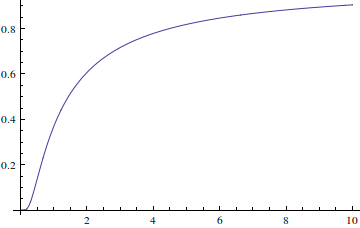
\includegraphics{img/05/lhopital.png}
\end{figure}

\begin{align}
  \lim_{x \to h} \frac{f(0+h)-f(0)}{h}
    &= \lim_{x \to h} \frac{e^{-\frac{1}{x}} - 0}{h} \\
    &= \lim_{x \to h} \frac{e^{-\frac{1}{x}}}{h} \\
  \intertext{apply l'Hopital's rule}
    &= \lim_{x \to h} \frac{\left(e^{-\frac{1}{x}}\right)'}{h} \\
  \intertext{This presents a problem becase}
  \left(e^{-\frac{1}{x}}\right)' &= \frac{1}{h^2}e^{-\frac{1}{x}}
  \intertext{leaving a harder problem:}
  \lim_{x \to h} \frac{e^{-\frac{1}{x}} - 0}{h}
    &= \lim_{x \to h} \frac{\frac{1}{h^2}e^{-\frac{1}{x}}}{h} \\
  \intertext{but we can rewrite as}
%  \lim_{x \to h} \frac{\frac{1}{h}}{e^{\frac{1}{h}}
%    &= \lim_{h \to 0^+} \frac{\left(\frac{-1}{h^2}\right)}{e^{\frac{1}{h}}(-\frac{1}{h^2})} \\
%    &= \lim_{h \to 0^+} \frac{1}{e^{\frac{1}{h}}}\cdot \frac{(-1/h^2)}{(-1/h^2)} \\
    &= \lim_{h \to 0^+} \text{TODO FINISH}
    % TODO FINISH ME FROM ONLINE NOTES.
\end{align}

\subsection{Another example}
\begin{align}
  \lim_{x \to 0} \frac{\sin x}{x} &= \lim_{x \to 0} \frac{ \cos x}{1} &= 1
  \intertext{Shown:}
  (\sin x)' &= \cos x
  \intertext{using}
  \lim_{x \to 0} \frac{\sin x}{x} = 1
\end{align}

\subsection{Example}

\begin{align}
  \lim_{x \to 0} \frac{1 - \cos(ax)}{1 - \cos x} &
  \intertext{$a = 0$}
  \lim_{x \to 0} \frac{1 - 1}{1 - \cos x}
    &= \lim_{x \to 0} \frac{0}{1 - \cos x} \\
    &= 0
  \intertext{$a \neq0$}
  \lim_{x \to 0} (1 - \cos(ax)) &= 0 \\
  \lim_{x \to 0} (1 - \cos(x)) &= 0 \\
  \lim_{x \to 0} \frac{ 1 - \cos(ax)}{1-\cos(x)}
    &= \lim_{x \to 0} \frac{a \sin(ax)}{\sin x} \exists ? \\
  &= \lim_{x \to 0} \frac{a^2\cos(ax)}{\cos x} \\
  &= a^2 \lim_{x \to 0} \frac{\cos(ax)}{\cos x} \text{does exist!} \\
  &= a^2
\end{align}


\section{Second and third derivatives}
If derivative of $f$ at $x$ is given by $f'(x)$ is $f'$ differentiable?
\begin{align}
  f(x) &= x^3 \\
  f'(x) &= 3x^2 \\
  f''(x) &= 6x \\
  f'''(x) &= 6 \\
\end{align}

% TODO include plots of concave up (convex) and concave down functions and
%label them as such

For all $x_1 < x_2$, $\lambda f(x_1) + (1-\lambda)f(x_2) \leq
f(\lambda x_1 + (1-\lambda)x_2)$ | $0 \leq \lambda \leq 1$ then a function is
said to be concave down

Then the following is equivalent:
1) $f$ is concave up on $[a,b]$
2) $f'$ is increasing on $[a,b]$
3) $f''(x) \geq 0$ on $[a,b]$

Then the following is equivalent:
1) $f$ is concave down on $[a,b]$
2) $f'$ is increasing on $[a,b]$
3) $f''(x) \leq 0$ on $[a,b]$
